\chapter{Basics}

Little-$o()$ notation is used to denote that some expression is small relative to some other value.

\begin{marginfigure}
\includegraphics[width=0.75\linewidth]{graphics/basics1.pdf}
\caption{$(1 + h )^3 = 1 + 3 h + o(h)$.}
\label{fig:basics1}
\end{marginfigure}
For example, if we say, as $h$ approaches $0$,
\begin{equation*}
(1 + h)^3 = 1 + 3 h + o(h)\,.
\end{equation*}
We mean that, as the magnitude of $h$ gets smaller, the magnitude of the difference between the left-hand side  $L = (1 + h )^3$ and the  right-hand side $R = 1 + 3 h$  is so small that, even when divided by $h$,  it is still small.

We can check this ratio empirically: 
\begin{table}
\caption[][0em]{$(1 + h )^3 = 1 + 3 h + o(h)$.}
\label{tab:basic1}
\begin{tabular}{|S[table-format=2.3]|S[table-format=2.9]|S[table-format=2.3]|S[table-format=2.11]|S[table-format=2.6]|}
\multicolumn{1}{c}{$h$} & 
\multicolumn{1}{c}{$L=(1+h)^3$} & 
\multicolumn{1}{c}{$R=1+3h$} & 
\multicolumn{1}{c}{$E=L-R$} &
\multicolumn{1}{c}{$r=\left|\frac{E}{h}\right|$} \\
\hline
0.1  & 1.331 & 1.3 & 0.031 & 0.31 \\
\hline
-0.01 & 0.970299 & 0.97 & 0.000299 & 0.0299 \\
\hline
0.001 & 1.003003001 & 1.003 & 0.00000030001 & 0.003001 \\
\hline
\end{tabular}
\end{table}

Notice how the ratio  $r=|E/h|$ shrinks as the magnitude of $h$ shrinks.  When we say an expression  $E$  is $o(h)$ as  $h \rightarrow 0$,  we mean the magnitude of $|E/h|$  gets small as the magnitude of $h$ gets small.

\begin{marginfigure}
\includegraphics[width=0.75\linewidth]{graphics/basics2.pdf}
\caption{As $k \rightarrow \infty$, $2k^3+5k^2-7k+3=2k^3+o(k^3)$.  Note how similar the curves are for large $k$.}
\label{fig:basics2}
\end{marginfigure}
\begin{marginfigure}
\includegraphics[width=0.75\linewidth]{graphics/basics3.pdf}
\caption{As $k \rightarrow \infty$, $2k^3+5k^2-7k+3=2k^3+o(k^3)$.  Note how dissimilar the curves are for small $k$.}
\label{fig:basics2}
\end{marginfigure}
The  $o()$  notation allows for more general expressions for the relative comparison of smallness,  such as  $o(h^2)$ or  $o(h \ln(h))$. In each case, we are saying that the expression in question is small in magnitude when divided by the expression in the $o()$  as the parameter ($h$ in this case) gets small in magnitude.

Here are some other examples to help get the idea.  You should check these with a calculator or spreadsheet.  We give a formal definition of the notation at the end of this section. 
 
As  $k \rightarrow \infty$,  $2k^3 + 5 k^2 - 7 k + 3 = 2k^3 + o (k^3 )$.     
 
This means, as the magnitude of  $k$ gets larger and larger, the cubic polynomial on the left is approximately the leading order term (term with the highest power of  $k$) plus an error small relative to the size of that term.   

\begin{table}
\caption{$2k^3 + 5 k^2 - 7 k + 3=2k^3+o(k^3)$.}
\label{tab:basic2}
\begin{tabular}{|S[table-format=4]|S[table-format=10]|S[table-format=10]|S[table-format=7]|S[table-format=10]|S[table-format=1.5]|}
\multicolumn{6}{c}{\vspace{1em}} \\
\multicolumn{1}{l}{$k$} & 
\multicolumn{1}{l}{$\begin{array}{c}L=2k^3+ 5 k^2 \\ - 7 k + 3\end{array}$} &\multicolumn{1}{l}{$R=2k^3$} & 
\multicolumn{1}{l}{$E=L-R$} &
\multicolumn{1}{l}{$\varepsilon(k)=k^3$} &
\multicolumn{1}{l}{$r=\left|\frac{E}{\varepsilon(k)}\right| $} \\
\hline
10  & 2433 & 2000 & 433 & 1000 & 0.43300 \\
-100 & -1949297 &  -2000000 & 50703 & -1000000 & 0.05070 \\
1000 & 2004993003 & 2000000000 & 4993003 & 1000000000 & 0.00499 \\
\hline
\end{tabular}
\end{table}

Notice how the error $E$ grows, but it is still small when compared to $\varepsilon(k) = k^3$.  

\section{Euler's constant, $e$.}
Euler's constant $e \approx \num{2.718281828459045}$ is fundamental for exponents and logarithms, just as  $\pi \approx \num{3.141592653589793} $ is fundamental in trigonometry.  It can be thought of as the value approximated by the expression $(1 + h)^{1/h}$ as $h \rightarrow 0$.

In $o()$ notation\footnote{Writing $1$ as  $h^0$ in the $o(h^0)$ may seem surprising, but it is a way of noting what parameter is getting small.}: as $h \rightarrow 0$, $(1 + h)^{1/h}=e+o(h^0)$.

This means, as the magnitude of  $h$ gets smaller and smaller, the expression on the left is approximately Euler's constant $e = \num{2.718281828459045}\ldots$, plus an error small relative to $h^0=1$.  
 
Here is a tabular comparison for some small values of $h$:  
 
\begin{table}
\caption{$(1 + h )^{1/h}=e+o(h^0)$.}
\label{tab:e}
\begin{tabular}{|S[table-format=2.6]|S[table-format=2.9]|S[table-format=1.8]|}
\multicolumn{1}{c}{$h$} & 
\multicolumn{1}{c}{$(1+h)^{1/h}$} &
\multicolumn{1}{c}{$r=\left|\frac{(1+h)^{1/h}-e}{1}\right| $} \\
\hline
0.01 & 2.704813829 & 0.0135 \\
-0.0001 & 2.718417755 & 0.000136 \\
0.000001 & 2.718280469 & 0.00000136 \\
\hline
\end{tabular}
\end{table}
\vspace{4em}
\begin{marginfigure}
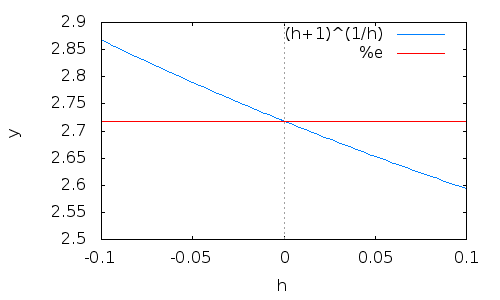
\includegraphics{graphics/e.pdf}
\caption{$(1 + h )^{1/h}=e+o(h^0)$.}
\label{fig:e}
\end{marginfigure}
   
\section{Sine.}
As $h \rightarrow 0$,  $\sin(x+h)=\sin(x)+\cos(x)h + o(h)$.    
\begin{marginfigure}
\includegraphics{graphics/sine.pdf}
\caption{$\sin(x+h)=\sin(x)+\cos(x) h+o(h)$ for $x=1$ and $\pi$.}
\label{fig:sine}
\end{marginfigure}
 
We will show this is true later, but, geometrically, it means that evaluating  $y=\sin(x)$ near $x$ is approximately a line\footnote{A line going through the point $(x_0,y_0)$ with slope $m$ is $y=y_0+m \cdot (x-x_0)$.} going through the point  $(x,\sin(x))$ with slope  $\cos(x)$.  

{\em This last example is really important.}  The idea that, near a given point  $x$,  many functions are well approximated by a line is a foundational idea of differential calculus.  
\begin{figure}
% \includegraphics{graphics/calc.pdf}
\caption{$\sin(x+h)=\sin(x)+\cos(x) h+o(h)$ for $x=1$ and $\pi$.}
\label{fig:calc}
\end{figure}

We call the slope of that approximating line  $f'(x)$, so that $f(x+h)=f(x)+f'(x)h+o(h)$.  For this example, we are saying that, if $f(x) = \sin(x)$, then  $f'(x)=\cos(x)$.  
 
The most important figure in calculus.  For many functions, the value near a given point  x is well approximated by a line called the tangent line of  f (x)  at  x with slope  f ′ (x).     As an  
equation: as  h → 0 ,   f (x + h ) = f (x) + f ′ (x)h + o (h).     Such functions are called differentiable at  x .  
 
Always writing “as  h → 0 "  is tedious.  It will be clear from the  o ()  notation which parameter we  
consider large or small. 
 
Formalities
E | is as small as we choose,  
An expression  E    is  o (ε(h))  as  h → 0 , means the ratio  r = || ε(h)
|
provided we force the magnitude of  h to be small enough (but not zero).  Specifically, for  
E | < r .  
any bound   r b > 0 ,  there exists an 
 
h b > 0 ,  so that, if  0 < | h | < h b ,  then  || ε(h)
| b
 
 
 
 
Redraw this in your notes so you remember the definition of little-o. 
 
 
E | = 0 .  
If you are familiar with limit notation, this can be written as  lim || ε(h)
|
h→0
 In terms of large parameters,  E = o (ε(k))    as  k → ∞   is the same as  E = o (ε(1/h))  as
   
h → 0 by means of the substitution  h = 1 /k.  
 
E | = 0 .  
If you are familiar with limit notation, this can be written as  lim || ε(k)
|
k→∞
 
Note that we divide  E  by 
  ε (h)  to get  r  in the above definition for some range of nonzero
 
 
values of  h .    So, for for any expression to be  o (ε(h)),   ε (h)  must be defined and nonzero  
for some range of nonzero values of  h .    We therefore restrict  ε (h)  to such admissible  
functions:   
 
For  ε (h)  to be admissible in  o (ε(h))  notation, there must exist some  h ε > 0  so  
that  ε (h)  is defined (finite) and nonzero for  0 < | h | < h ε .     
 
 
All we ask of  ε (h)  to be admissible, is that there is a range near zero (but we don’t  
care about at zero), where it is defined (finite) and nonzero.  This way we can 
divide  E    by  ε (h)  in this range to compute the ratio  r = | E/ε(h)|.  
 
 We only use admissible   ε (h)  in these notes.  In particular,  ε (h) = | h | p  is admissible for  
any value of  p ,  and   ε (h) = h p  is admissible for any integer value of  p .  
Summary
 
●
Little-o() notation is a way of describing an expression as small in comparison to 
some other value: saying  E  is 
  o (ε(h))  as  h → 0  means the ratio  r = | E/ε(h) |  can
 
 be made as small as desired provided the magnitude of  h is small enough (but  
not zero). 
 
●
Specifically,  E    is  o (ε(h))  as  h → 0  means:  
 
For any  r b > 0 ,  there exists 
 
h b > 0 ,  so that:   
E | < r .  
|
 If  0 < | h | < h b ,  then  | ε(h)
| b
 
● E  is 
  o (ε(k))    as  k → ∞   means  E is 
  o (ε(1/h))  as  h = 1 /k → 0 .  
● For differentiable functions, the value  f (x + h )  near a given point  x is well  
approximated by a line called the tangent line of  f (x)  at  x with slope  f ′ (x).    
● As  h → 0 ,   (1 + h ) (1/h) = e + o (h 0 ),  where  e ≈ 2 .718  is Euler’s constant.
 
 
● Because an expression  E  is divided by 
 
ε (h) in the definition of  o (ε(h)),   ε (h)  is  
admissible in  o (ε(h))  only if it is defined and nonzero for small enough nonzero  
h :  there must exist  h ε > 0  so that  ε (h)  is defined (finite) and nonzero for  
0 < | h | < h ε .     
●  We only use admissible   ε (h)  in these notes.  In particular,  ε (h) = | h | p  is  
admissible for any value of  p ,  and   ε (h) = h p  is admissible for any integer value of  
p.
